\documentclass[10pt,a4paper]{article}
% usepackages
\usepackage[latin1]{inputenc}
\usepackage[english]{babel}
% math
\usepackage{amsmath}
\usepackage{amsfonts}
\usepackage{amssymb}
\usepackage{mathtools}
\usepackage{latexsym}
% formatting
\usepackage{parskip}
\usepackage{fullpage}
\usepackage{pgf,tikz}
\usepackage{mathrsfs}
\usetikzlibrary{arrows}
\pagestyle{empty}
% graphics
%\usepackage[pdftex]{graphicx}
\usepackage{caption}
\usepackage{subcaption}
%\usepackage[all]{xy}

%\usepackage[below,section]{placeins} % the one below is better for short assignments
\usepackage{float} % provides H as float placement specifier
% extras
\usepackage[pdftex,a4paper,colorlinks=true,urlcolor=blue]{hyperref}
\urlstyle{same}
\usepackage{moreverb} %\verbatimtabinput{filename.py} preserves indentation
\usepackage{cite}
\pagenumbering{arabic}

%Numbering first level list roman (i,ii,iii) instead of arabic (1,2,3)
% options are \roman \Roman \alph \Alph \arabic
\renewcommand{\theenumi}{\roman{enumi}} 
\renewcommand{\theenumii}{\roman{enumii}}
\newcommand{\Int}{\int\limits}
% Also achieved with the enumerate package
\usepackage{enumerate}
%\numberwithin{equation}{section}%

% author/title details
\author{Alice NANYANZI (\href{mailto:alicenanyanzi@aims.ac.za}{alicenanyanzi@aims.ac.za})}
% \title{Course Title: Assignment X}
\title{Long range interactions in Image segmentation}
\begin{document}
\maketitle
Here we compare image segmentation on a toy example of a lattice using various transforms of k-path Laplacian. 

\section{Mellin transform of k-path Laplacian}
First we consider Mellin transform given by

\begin{equation*}
\mathcal{L}_{M,s} = \sum_{k=1}^{\infty}\frac{1}{k^s} L_k
\end{equation*}



\begin{figure}[H]
	\centering
	\begin{subfigure}[b]{0.45\textwidth}
		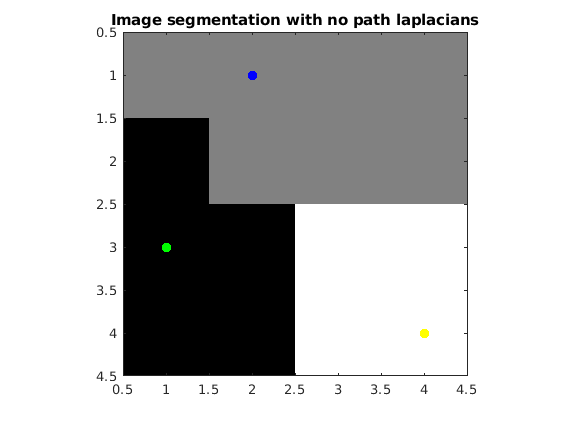
\includegraphics[width=\textwidth]{segmentation-images/4by4longrange1-s4.png}
		\caption{k=1}
	\end{subfigure}
	\begin{subfigure}[b]{0.45\textwidth}
		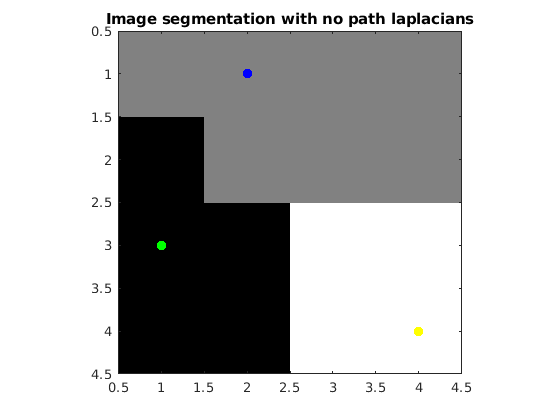
\includegraphics[width=\textwidth]{segmentation-images/4by4longrange2-s2.png}
		\caption{k up to 2}
	\end{subfigure} \\
    \begin{subfigure}[b]{0.45\textwidth}
    	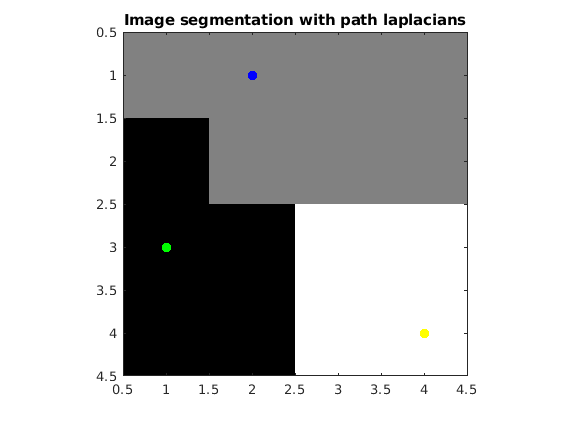
\includegraphics[width=\textwidth]{segmentation-images/4by4longrange3-s2.png}
    	\caption{k up to 3}
    \end{subfigure}
    \begin{subfigure}[b]{0.45\textwidth}
    	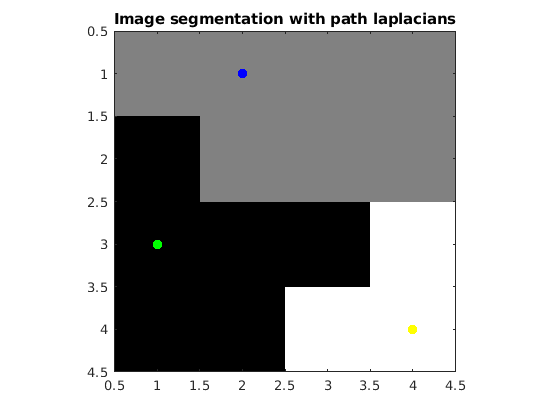
\includegraphics[width=\textwidth]{segmentation-images/4by4longrange6-s2.png}
    	\caption{k up to 6(diameter)}
    \end{subfigure}\\
    \begin{subfigure}[b]{0.45\textwidth}
    	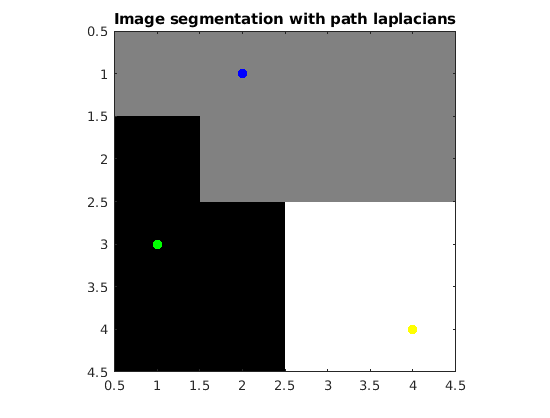
\includegraphics[width=\textwidth]{segmentation-images/4by4longrange3-s4.png}
    	\caption{k up to 3}
    \end{subfigure}
    \begin{subfigure}[b]{0.45\textwidth}
    	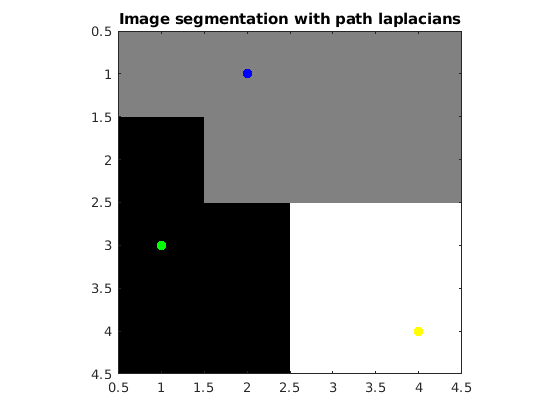
\includegraphics[width=\textwidth]{segmentation-images/4by4longrange6-s4.png}
    	\caption{k up to 6(diameter)}
    \end{subfigure}  

	\caption{ A $4 \times 4$ lattice representing pixels of an image each of intensity $1$. We carry out image segmentation by assigning each pixels to the label(either blue, yellow or green) for which the probability of a random walker starting at any pixel p first reaches the label is highest.We use Mellin transforms with $s=2$, for the first and second law. The third row corresponds to $s=4$ } 
\end{figure}

\vspace*{10mm}

Here we investigate how the segmentation happens on an $8 \times 8$ lattice.

%\begin{figure}[!h]
%	\centering
%	\begin{subfigure}[b]{0.45\textwidth}
%		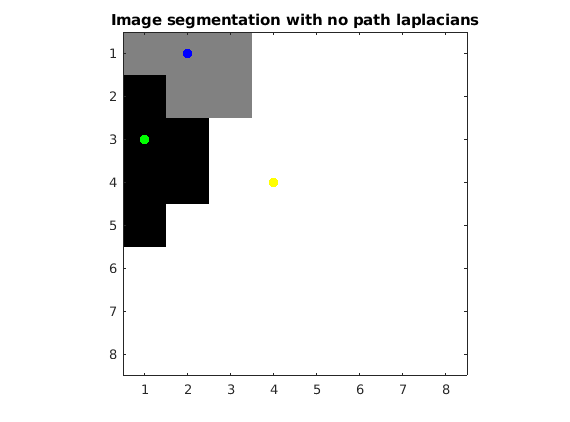
\includegraphics[width=\textwidth]{segmentation-images/8by8longrange1-s4.png}
%		\caption{k=1}
%	\end{subfigure}
%	\begin{subfigure}[b]{0.45\textwidth}
%		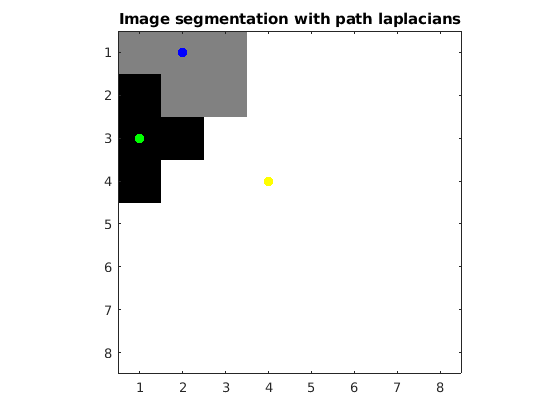
\includegraphics[width=\textwidth]{segmentation-images/8by8longrange2-s4.png}
%		\caption{k up to 3}
%	\end{subfigure} \\
%	\begin{subfigure}[b]{0.45\textwidth}
%		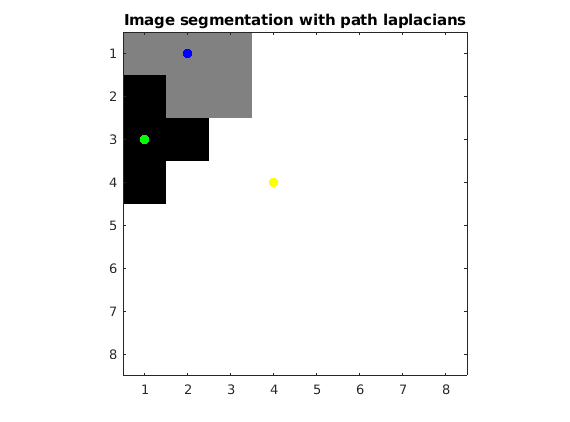
\includegraphics[width=\textwidth]{segmentation-images/8by8longrange6-s4.png}
%		\caption{k up to 4}
%	\end{subfigure}
%	\begin{subfigure}[b]{0.45\textwidth}
%		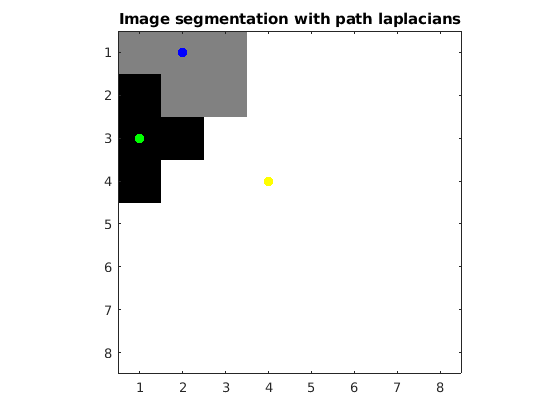
\includegraphics[width=\textwidth]{segmentation-images/8by8longrange14-s4.png}
%		\caption{k up to 8 (diameter)}
%	\end{subfigure}
%	
%	\caption{ A $6 \times 6$ lattice representing pixels of an image each of intensity $1$. We carry out image segmentation by assigning each pixels to the label(either blue, yellow or green) for which the probability of a random walker starting at any pixel p first reaches the label is highest.} 
%\end{figure}

\begin{figure}[!h]
	\centering
	\begin{subfigure}[b]{0.45\textwidth}
		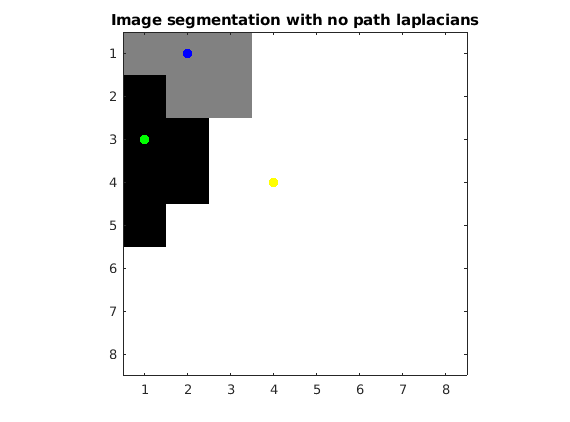
\includegraphics[width=\textwidth]{segmentation-images/8by8longrange1-s4.png}
		\caption{k=1}
	\end{subfigure}
	\begin{subfigure}[b]{0.45\textwidth}
		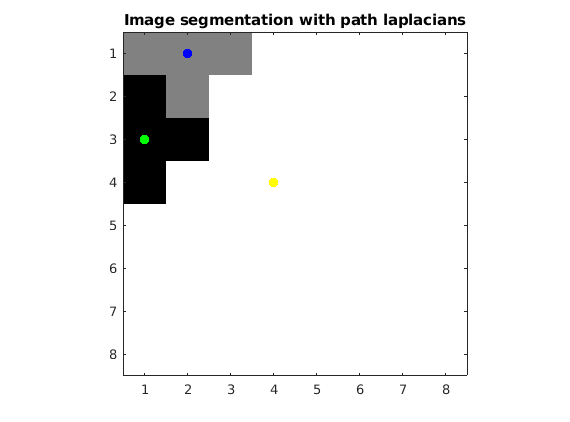
\includegraphics[width=\textwidth]{segmentation-images/8by8longrange3-s2.png}
		\caption{k up to 3}
	\end{subfigure} \\
    \begin{subfigure}[b]{0.45\textwidth}
    	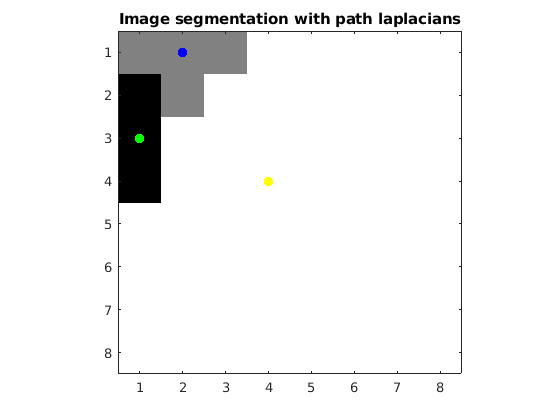
\includegraphics[width=\textwidth]{segmentation-images/8by8longrange6-s2.png}
    	\caption{k up to 6}
    \end{subfigure}
    \begin{subfigure}[b]{0.45\textwidth}
    	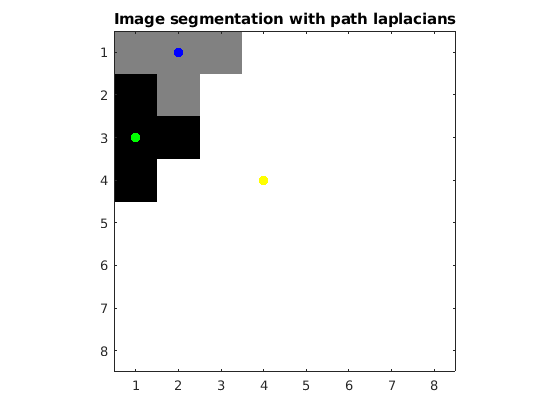
\includegraphics[width=\textwidth]{segmentation-images/8by8longrange14-s2.png}
    	\caption{k up to 14}
    \end{subfigure} \\
	\begin{subfigure}[b]{0.45\textwidth}
		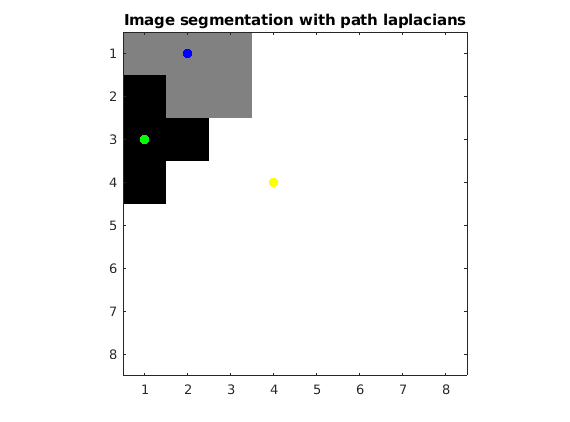
\includegraphics[width=\textwidth]{segmentation-images/8by8longrange6-s4.png}
		\caption{k up to 6}
	\end{subfigure}
	\begin{subfigure}[b]{0.45\textwidth}
		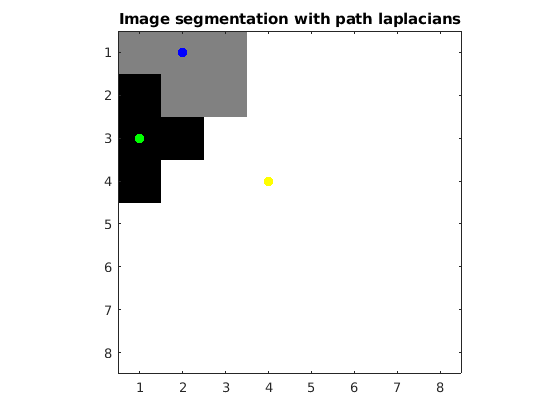
\includegraphics[width=\textwidth]{segmentation-images/8by8longrange14-s4.png}
		\caption{k up to 14 (diameter)}
	\end{subfigure}
	
	\caption{ Illustration of segmentation, figure (a) corresponds to results by the Laplacian matrix,L while figures(b),(c), and (d) follows from k-path Laplacians of the Mellin transform with $s=2$. On the otherhand, figures(b),(c), and (d) follows from k-path Laplacians of the Mellin transform with $s=4$} 
\end{figure}

\vspace*{2cm}
For a $16 \times 16 $ matrix, we have the following illustrations.

\begin{figure}[H]
	\centering
	\begin{subfigure}[b]{0.45\textwidth}
		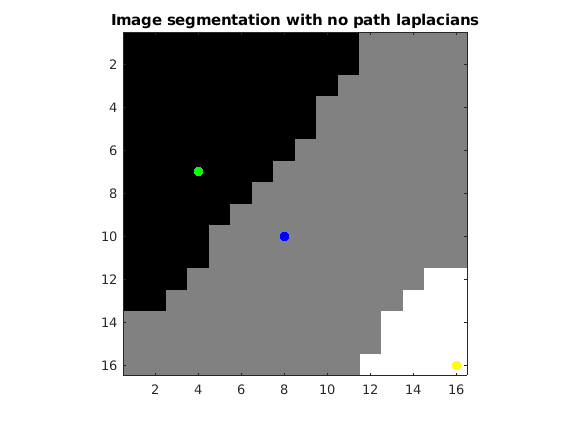
\includegraphics[width=\textwidth]{segmentation-images/16by16longrange1-s2.png}
		\caption{k=1}
	\end{subfigure}
	\begin{subfigure}[b]{0.45\textwidth}
		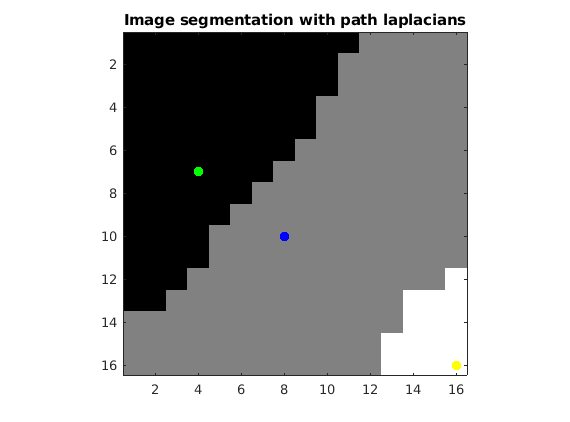
\includegraphics[width=\textwidth]{segmentation-images/16by16longrange2-s2.png}
		\caption{k up to 2}
	\end{subfigure} \\
	\begin{subfigure}[b]{0.45\textwidth}
		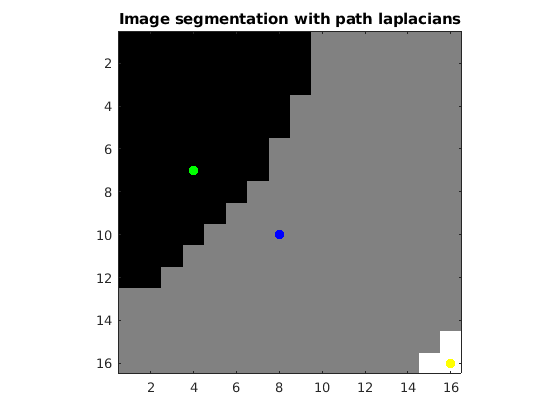
\includegraphics[width=\textwidth]{segmentation-images/16by16longrange6-s2.png}
		\caption{k up to 6}
	\end{subfigure}
	\begin{subfigure}[b]{0.45\textwidth}
		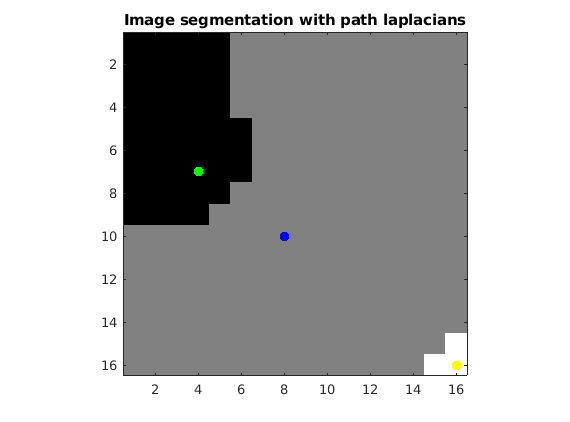
\includegraphics[width=\textwidth]{segmentation-images/16by16longrange14-s2.png}
		\caption{k up to 14}
	\end{subfigure}\\
	\begin{subfigure}[b]{0.45\textwidth}
		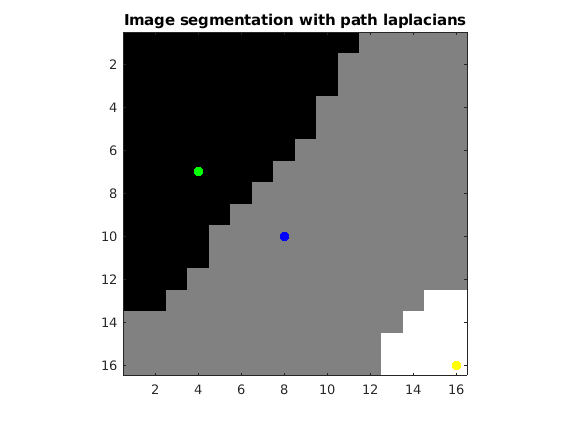
\includegraphics[width=\textwidth]{segmentation-images/16by16longrange6-s4.png}
		\caption{k up to 6}
	\end{subfigure}
	\begin{subfigure}[b]{0.45\textwidth}
		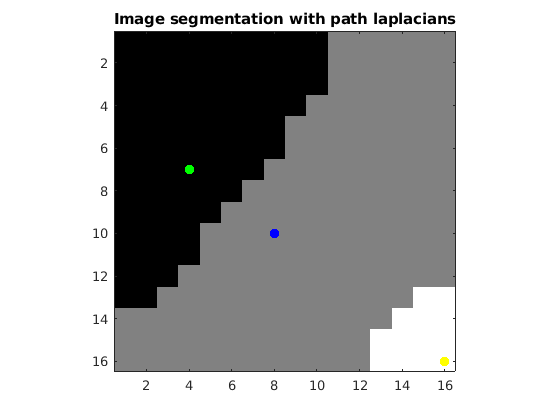
\includegraphics[width=\textwidth]{segmentation-images/16by16longrange14-s4.png}
		\caption{k up to 14}
	\end{subfigure}  
	
	\caption{ A $16 \times 16$ lattice representing pixels of an image each of intensity $1$. We carry out image segmentation by assigning each pixels to the label(either blue, yellow or green) for which the probability of a random walker starting at any pixel p first reaches the label is highest.We use Mellin transforms with $s=2$, for the first and second law. The third row corresponds to $s=4$ } 
\end{figure}




\section{Laplace transform of k-path Laplacian}

When we consider Laplace transformed k-path Laplacian given by 

\begin{equation*}
\mathcal{L}_{L,\lambda} = \sum_{k=1}^{\infty} e^{-\lambda k} L_k
\end{equation*}
\end{document}
